\section{Tipus de fractals}
Dins de les fractals tenim diferents tipus, en podem destacar tres: les fractals naturals, les geomètriques i les algebraiques.

\subsection{Les fractals naturals}
Aquestes fractals es caracteritzen pel fet que apareixen a la natura. No segueixen cap forma geomètrica ni cap norma, simplement cada cop que ens apropem podem veure com es va repetint.
\newline

\begin{figure}[h]
    \centering
    \begin{minipage}{.5\textwidth}
      \centering
      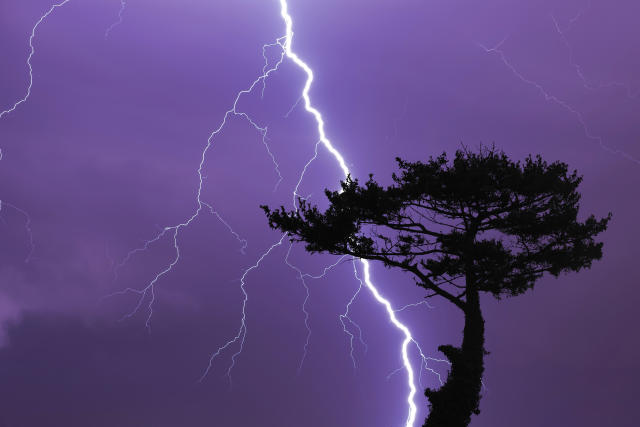
\includegraphics[width=.8\linewidth]{imatges/dos-fractals-naturals.jpg}
      \captionof{figure}{Un arbre i un llampec.}
      \label{fig:arbre_i_llampec}
    \end{minipage}%
    \begin{minipage}{.5\textwidth}
      \centering
      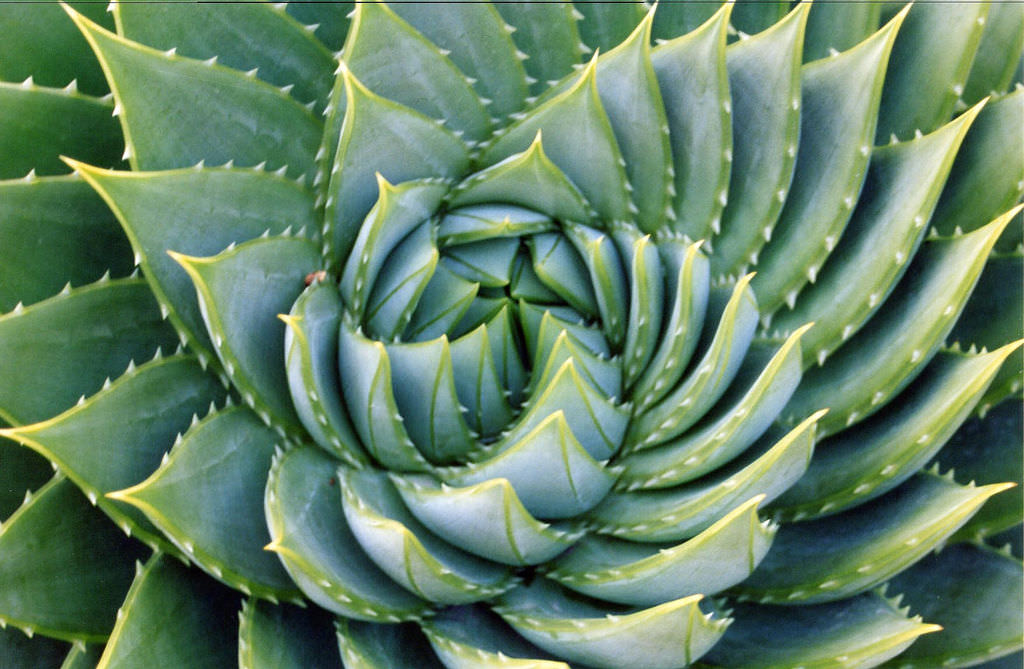
\includegraphics[width=.8\linewidth]{imatges/planta-espiral.jpg}
      \captionof{figure}{Planta creixent en espiral.}
      \label{fig:espiral}
    \end{minipage}
\end{figure}
\noindent
Com a exemples tenim l'arbre i el llampec en la figura \ref{fig:arbre_i_llampec}. Però a més a més, en la figura \ref{fig:espiral} podem veure una planta que creix en espiral. Aquesta segueix la Seqüència de Fibonacci i es pot veure com un cas especial de similitud amb ella mateixa.

\subsection{Les fractals geomètriques}
Aquestes fractals són els més senzills d'entendre, ja que simplement són ells mateixos repetits. Segueixen unes normes molt bàsiques, que canvien en cada fractal, i podem dir amb seguretat que no han estat generats arbitràriament, cosa que no podem estar tan segurs de pensar en les fractals algebraiques. \n
L'única diferència que hi ha entre una fractal geomètrica i una d'algebraica és el seu punt de partida. Doncs aquests s'inicien amb una forma geomètrica. \n
En la figura \ref{fig:sierpinski} podem veure el triangle de Sierpinski. El seu punt inicial és un triangle equilàter. Aquest triangle està ple i és emplenat amb un altre triangle equilàter buit al centre de la manera que aquest triangle sigui igual de gran que els tres triangles que es formen al seu costat. \n
En canvi, en la figura \ref{fig:arbre_fractal} podem veure una fractal en forma d'arbre. Aquest ha estat generat agafant una figura inicial en forma de Y i posant-hi, en la bifurcació d'aquesta figura, la mateixa, de mode que el tronc del model agregat és també la bifurcació de la figura inicial. Si aquesta acció és repetida suficients vegades per a no notar ja un canvi, tindrem la figura \ref{fig:arbre_fractal}.

\begin{figure}[h]
    \centering
    \begin{minipage}{.5\textwidth}
      \centering
      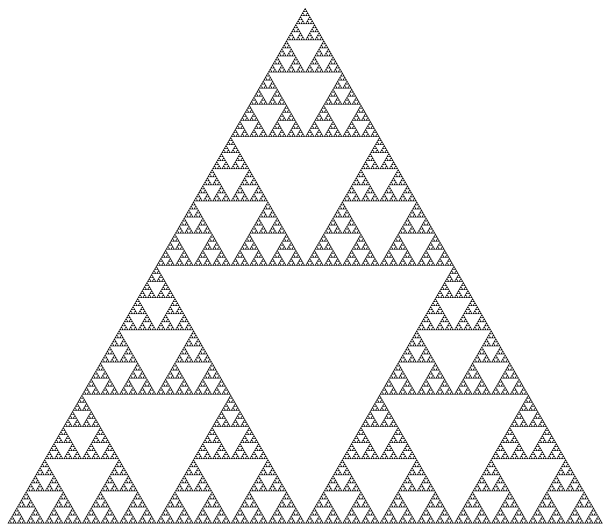
\includegraphics[width=.8\linewidth]{imatges/sierpinski.jpg}
      \captionof{figure}{Triangle de Sierpinski.}
      \label{fig:sierpinski}
    \end{minipage}%
    \begin{minipage}{.5\textwidth}
      \centering
      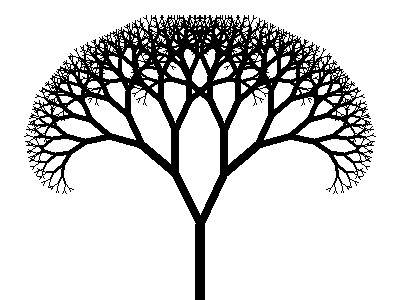
\includegraphics[width=.8\linewidth]{imatges/fractal-tree.jpg}
      \captionof{figure}{Fractal en forma d'arbre.}
      \label{fig:arbre_fractal}
    \end{minipage}
\end{figure}
\noindent

\subsection{Les fractals algebraiques}
Aquestes fractals, tal i com he anomenat abans, podriem pensar que han estat generades arbritàriament si ens limitem a veure una imatge. Aquestes fractals no son més que una equació de nombres complexos iterada infinitament. Si al posar un número del pla complex aquest no tendeix a infinit, aquest nombre forma part de la fractal. \n
Les fractals algebraiques no es limiten a una simple equació. També tenen les seves normes. Com ara començar a iterar el nombre igualant $z_0 = 0$ i fent que $c = v_{punt}$. Si l'equació d'aquesta fractal és $f(z) = z^2 + c$, s'anomena Conjunt de Mandelbrot.

\subsubsection{Conjunt de Mandelbrot}
Seguint amb l'exemple anterior, diguem que volem calular el nombre $z = -1 + 0i$ (si els nombres complexos no tenen part imaginaria, com aquest cas, els podem tractar com a nombres reals):
\[f(0) = 0^2 + c \; c = (-1, 0)\]
\[f_0(0) = 0^2 - 1 = -1\]
\[f_1(-1) = (-1)^2 -1 = 0\]
\[f_2(0) = 0^2 - 1 = -1\]
Com es pot veure, ja que el nombre no tendeix a infinit, doncs va saltant de 0 a -1, el nombre complex $z = -1 + 0i$, forma part del conjunt de Mandelbrot. Donant el nombre $z = 1 + 0i$:
\[f_0(0) = 0^2 + 1 = 1\]
\[f_1(1) = 1^2 + 1 = 2\]
\[f_2(2) = 2^2 + 1 = 5\]
\[f_3(5) = 5^2 + 1 = 26\]
Amb aquest nombre no hem tingut tanta sort! Cada com que iterem aquest nombre es fa cada cop més i més gran. Això ens indica que aquest nombre tendeix a infinit. Per tant, no forma part del confunt de Mandelbrot. Si fem això per cada punt, obtenim aquesta imatge:

\begin{figure}[h!]
    \centering
    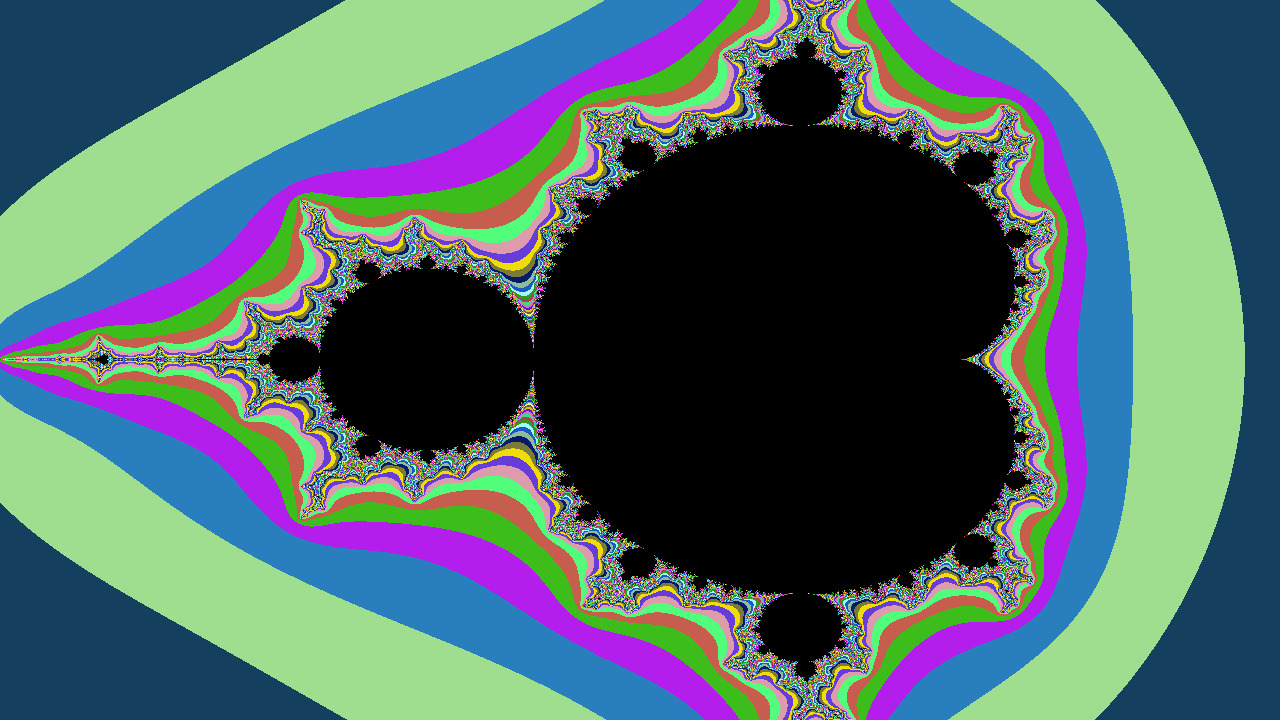
\includegraphics[width=.65\linewidth]{imatges/Captured_On_Sat_Aug__7_16-04-10_2021-.jpg}
    \captionof{figure}{Representació del conjunt de Mandelbrot.}
    \label{fig:mandelbrot_example}
\end{figure}

\subsubsection{Conjunt de Julia}
El conjunt de Julia segueix la mateixa funció que el de Mandelbrot. Però en aquest cas canviem la norma. Fixem $c$ a un nombre arbritari que nosaltres escollim i canviem $z_0$ pel punt on s'està iterant. Donem un exemple, tractarem amb nombres reals, doncs és més senzill:
\[c = 1 + 0i\]
Donem els punts $z_{0_1} = 1 + 0i$ i $z_{0_2} = -1 + 0i$: \newline
\begin{center}
\begin{tabularx}{0.8\textwidth} {
  >{\centering\arraybackslash}X |
  >{\centering\arraybackslash}X}
  \(f_{1_1}(z_{0_1}) = 1^2 + 1 = 2\) \vspace*{3mm} & \(f_{2_1}(z_{0_2}) = (-1)^2 + 1 = 2\) \\
  \(f_{1_2}(2) = 2^2 + 1 = 5\) \vspace*{3mm} & \(f_{2_2}(2) = 2^2 + 1 = 5\) \\
  \(f_{1_3}(5) = 5^2 + 1 = 26\) & \(f_{2_3}(5) = 5^2 + 1 = 26\)
\end{tabularx}
\end{center}
\noindent \newline
En aquest cas podem veure com els dos nombres no formen part del conjunt de Julia per $c = 1 + 0i$. \n
Fixem $c$ a un altre nombre:
\[c = -1 + 0i\]
Donem els mateixos punts $z_{0_1} = 1 + 0i$ i $z_{0_2} = -1 + 0i$: \newline
\begin{center}
\begin{tabularx}{0.8\textwidth} {
  >{\centering\arraybackslash}X |
  >{\centering\arraybackslash}X}
  \(f_{1_1}(z_{0_1}) = 1^2 - 1 = 0\) \vspace*{3mm} & \(f_{2_1}(z_{0_2}) = (-1)^2 + 1 = 0\) \\
  \(f_{1_2}(0) = 0^2 - 1 = -1\) \vspace*{3mm} & \(f_{2_2}(0) = 0^2 - 1 = -1\) \\
  \(f_{1_3}(-1) = (-1)^2 - 1 = 0\) & \(f_{2_3}(-1) = (-1)^2 - 1 = 0\)
\end{tabularx}
\end{center}
\noindent \newline
Ara podem veure que els dos nombres formen part del conjunt de Julia per $c = -1 + 0i$. \n
Si ho fesim per cada punt del pla obtindriem aquestes imatges:
\begin{figure}[h]
    \centering
    \begin{minipage}{.5\textwidth}
      \centering
      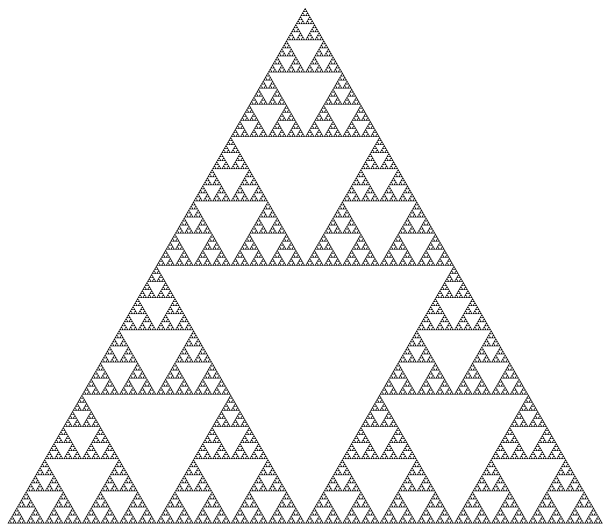
\includegraphics[width=.8\linewidth]{imatges/sierpinski.jpg}
      \captionof{figure}{Per $c = $.}
      \label{fig:Julia_example_}
    \end{minipage}%
    \begin{minipage}{.5\textwidth}
      \centering
      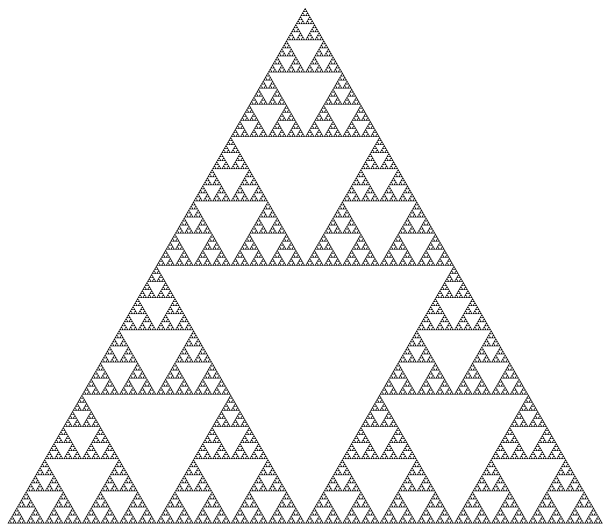
\includegraphics[width=.8\linewidth]{imatges/sierpinski.jpg}
      \captionof{figure}{Per $c = $.}
      \label{fig:Julia_example_}
    \end{minipage}
\end{figure}
\noindent
